\documentclass[12pt,a4paper,oneside]{article}

\usepackage{graphicx}
\usepackage{amsmath}

\begin{document}

\begin{titlepage}

\centering
	
\includegraphics[width=4cm]{logo.jpg}
	\vfill
    {\bfseries\Large
        DT2118 Lab1: Feature extraction
        \vskip1cm
        Thomai Stathopoulou\\
        \vskip1cm
        April 18th, 2015
    }    
   \vfill
\end{titlepage}

\section{Mel Frequency Cepstrum Coefficients}

In the first part of the Lab, the Mel Frequency Cepstrum Coefficients (MFCCs) of different speech signals are to be computed. In the following sections the different steps are described and commented upon.

\subsection{Enframe}

Since the sampling rate of the signals $f_s$ is known, it is easy to calculate the period of the sampling procedure as: $T = \frac{1}{f_s}$. The signal samples that we have, are sampled at a frequency $f_s = 20kHz$, hence the period is $T = 0.05 ms$. This means that a window length of $20ms$ and a window shift of $10ms$ are translated into $400$ and $200$ samples respectively. When the window reaches the end of the signal, the remaining samples that don't fit entirely in a window, are discarded. Figure \ref{fig:frames} shows the results of the $enframe$ function.

\begin{figure}[h]
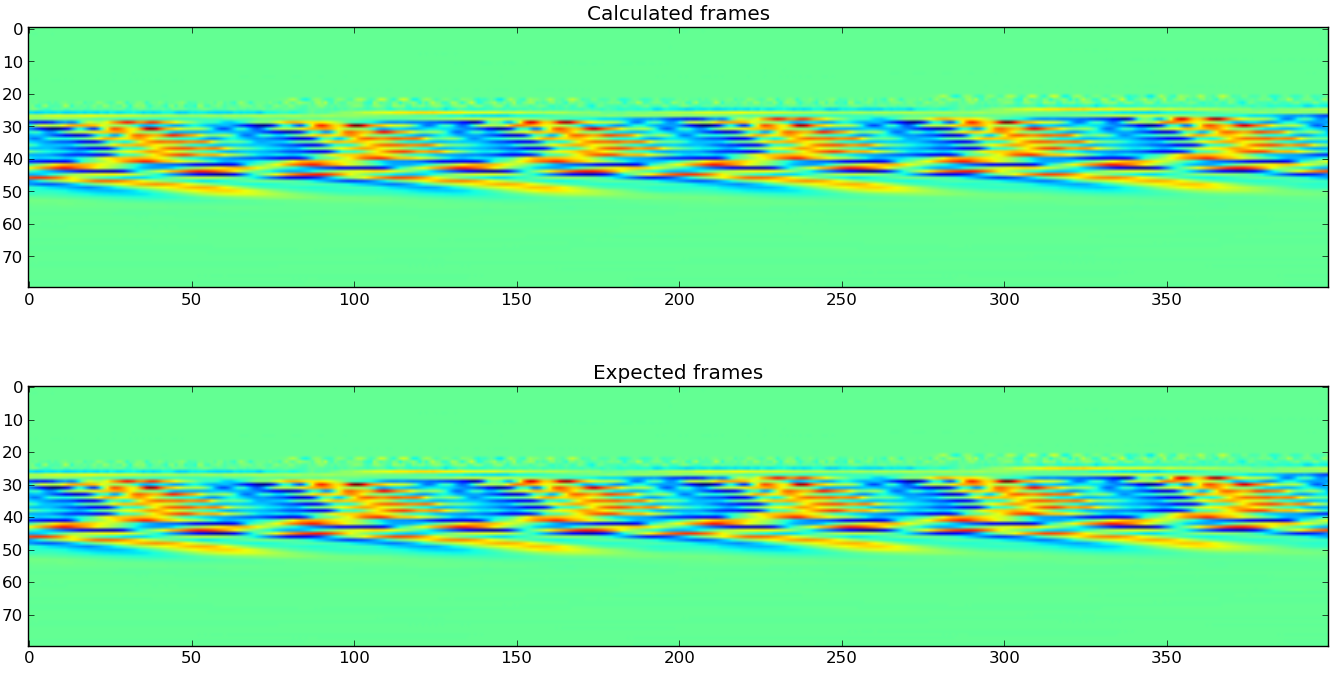
\includegraphics[scale=0.4]{../frames.png}
\caption{The frames from the ``Example'' Signal as were calculated by the \textit{enframe} function and as were expected}
\label{fig:frames}
\end{figure}


\subsection{Pre-emphasis}
When a low-frequency signal is sampled at a high frequency, its samples tend to change slowly and smoothly. For that reason, the signal is usually pre-emphasized. This means that from every sample we subtract the value of the previous one scaled by a factor $\alpha$:
\begin{equation} \label{eq:preeph}
y[n] = x[n] - \alpha x[n - 1]
\end{equation}
where usually $\alpha = 0.97$.

By subtracting, we remove the part of the sample that did not change in relation to its adjacent samples (the change can be parametrized by $\alpha$) and so what remains is the part of the signal that changes rapidly.

Python's $lfilter$ function implements an Infinite Impulse Response (IIR) filter. It therefore produces the following signal:

\begin{equation}
\begin{split}
a_0 y[n] = b_0 x[n] + b_1 x[n-1] + \dots + b_{nb} x[n-n_b]\\
	 - (a_1 y[n-1] + \dots + a_{na} y[n-n_a])
\end{split}
\end{equation}
In order to achieve the pre-emphasis equation we have to set $a_0 = 1$, $a_1, \dots, a_{na} = 0$, $b_0 = 1$, $b_1 = -\alpha = - 0.97$ and $b_2, \dots, b_{nb} =0$. By removing the $a$ from the filter, we basically remove the factor that renders the response an infinite signal. We now have a Finite Impulse Response (FIR) filter in the form of Equation \ref{eq:preeph}. Figure \ref{fig:preemph} shows the results of the $preemp$ function.

\begin{figure}[h]
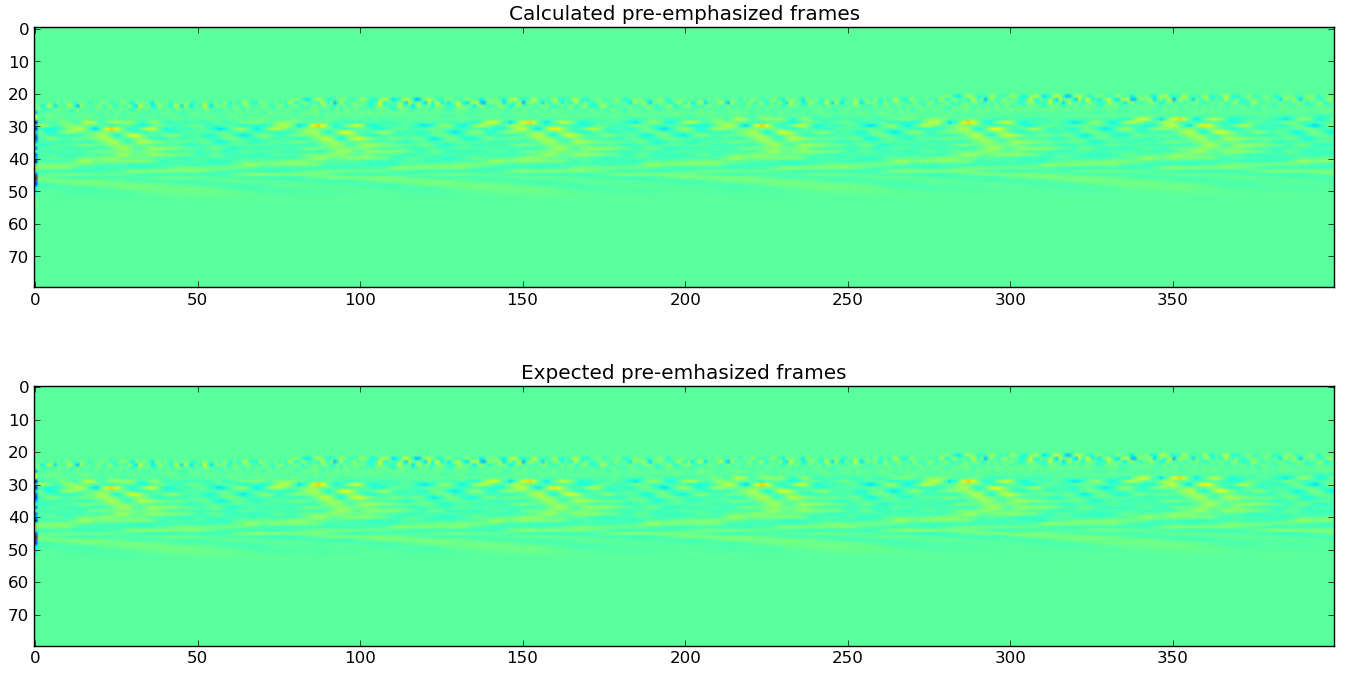
\includegraphics[scale=0.4]{../preemph.png}
\caption{The pre-emphasized frames from the ``Example'' Signal as were calculated by the \textit{preemp} function and as were expected}
\label{fig:preemph}
\end{figure}

\subsection{Hamming Window}
When Discrete Fourier transform is calculated for a finite signal, the signal is replicated infinite times, in order for it to look like an infinite signal. If the beginning and ending of the signal do not match, this will look like a discontinuity in the infinite signal and it will produce an incorrect Fourier transform, especially in the high frequency area.

\begin{figure}[h]
\centering
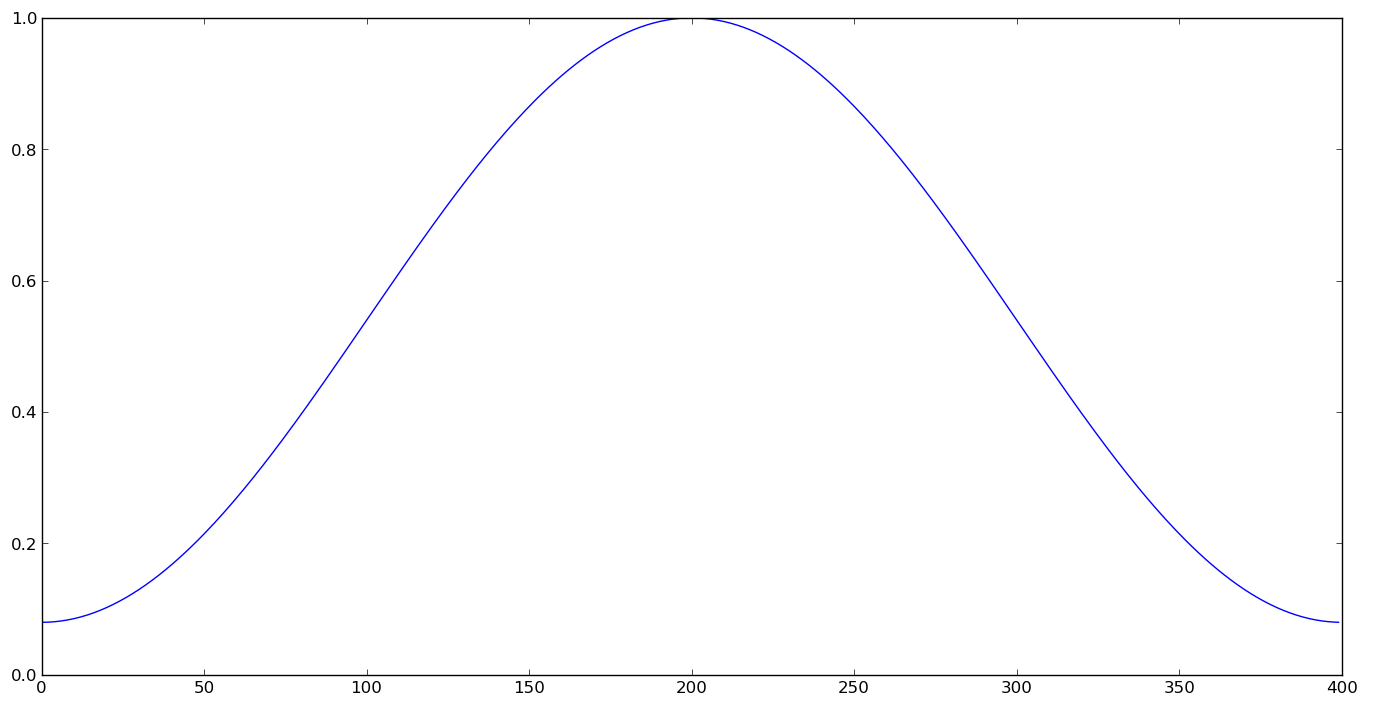
\includegraphics[scale=0.3]{../hamming.png}
\caption{Hamming window applied to the frames}
\label{fig:hamming}
\end{figure}

By applying the Hamming window (Fig. \ref{fig:hamming}) to the original signal, we try to smooth the transition from each repetition of the signal, so that it looks more like an infinite signal and less like one finite signal repeated infinite times. Figure \ref{fig:windowed} shows the frames, after the Hamming window was applied.

\begin{figure}[h]
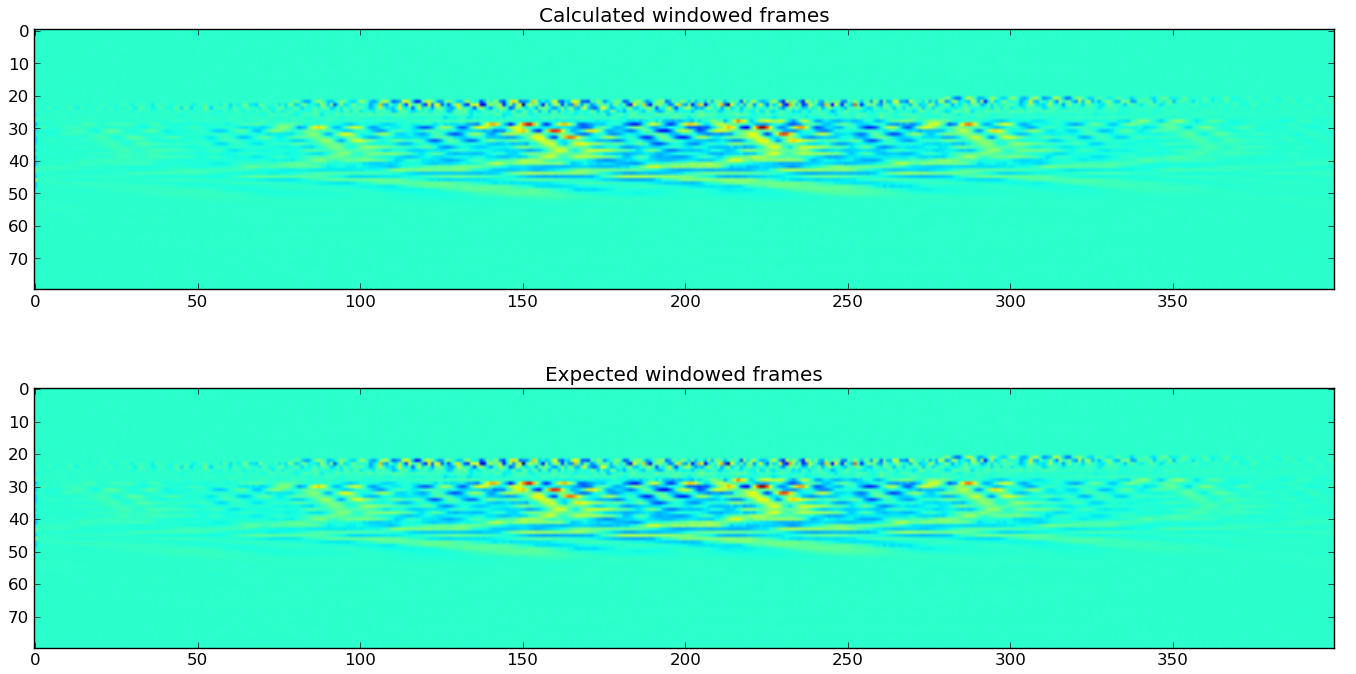
\includegraphics[scale=0.4]{../windowed.png}
\caption{The windowed frames after the application of the Hamming window}
\label{fig:windowed}
\end{figure}

\subsection{Fast Fourier Transform}
When calculating the Discrete Fourier Transform of a finite signal sampled at frequency $f_s$, the spectrum of the covers frequencies from $0$ to $f_{max}$ and back to $0$ (or more usually from $-f_{max}$ to $f_{max}$). This $2f_{max}$ bandwidth of the spectrum is repeated with frequency $f_s$. According to the Sampling Theorem, $f_{max} \leq \frac{f_s}{2}$, otherwise we have the phenomenon of the aliasing (Figure \ref{fig:alias} C), where the spectrum of the signal is distorted and the full reconstruction of the original image becomes impossible.

\begin{figure}[h]
\centering
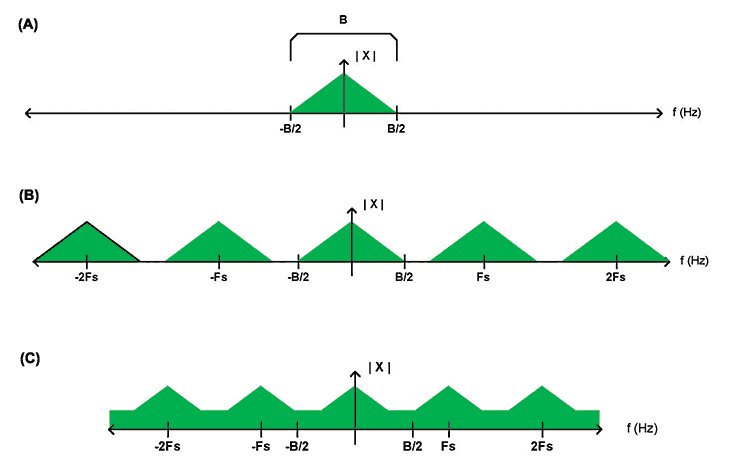
\includegraphics[scale=0.5]{fig5_big.png}
\caption{Spectrum of a signal and the phenomenon of aliasing [\scriptsize{Source: http://archives.sensorsmag.com/articles/0103/38/}]}
\label{fig:alias}
\end{figure}

For this Lab, since $f_s = 20kHz$, then we have the constraint: $f_{max} \leq 10kHz$. Figures \ref{fig:spec} and \ref{fig:logspec} show the squared modulus and the base 10 logarithm of the Fast Fourier Transform respectively.

\begin{figure}
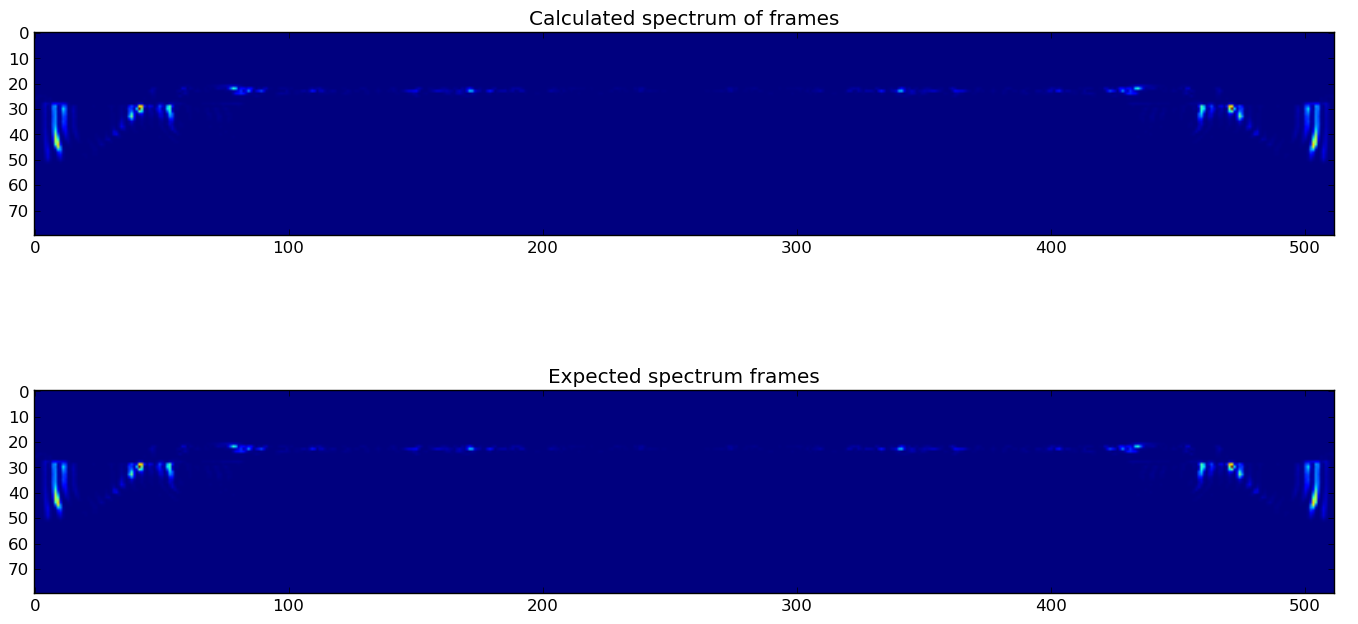
\includegraphics[scale=0.4]{../spec.png}
\caption{The spectrum of the frames.}
\label{fig:spec}
\end{figure}

\begin{figure}
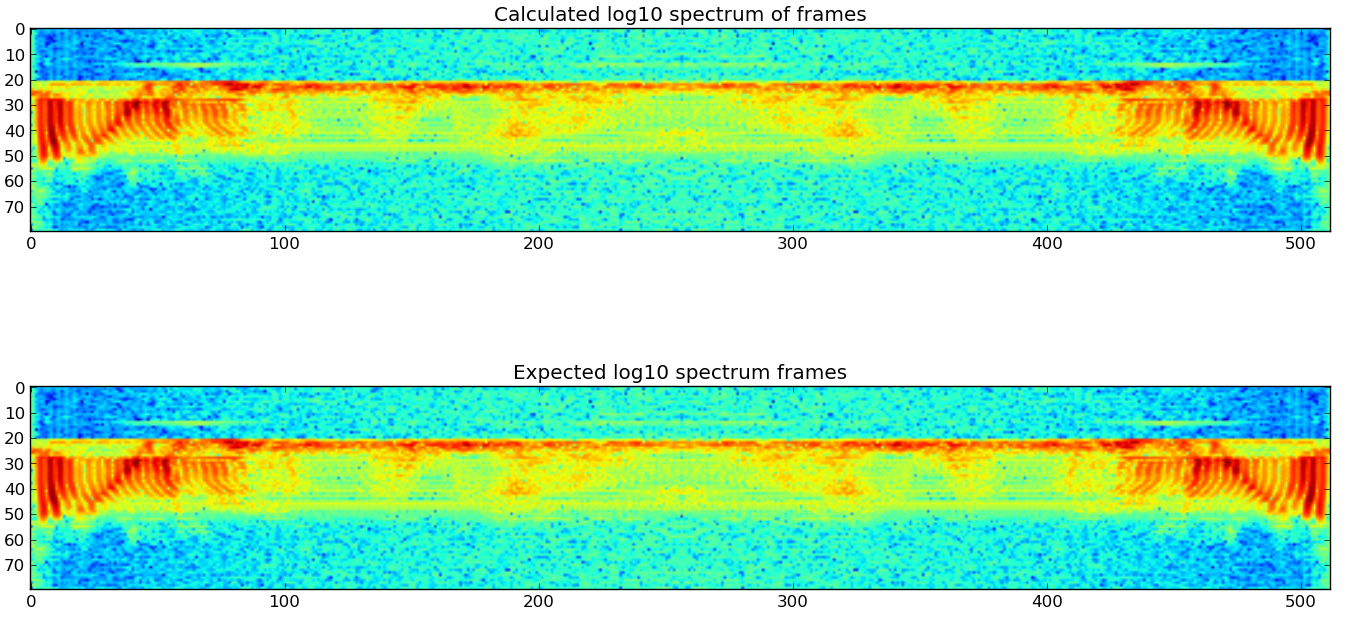
\includegraphics[scale=0.4]{../logspec.png}
\caption{The base 10 logarithm of the spectrum of the frames.}
\label{fig:logspec}
\end{figure}

\subsection{Mel filterbank}
The human ear resolves frequencies non-linearly across the audio spectrum and empirical evidence suggests that designing a front-end to operate in a similar non-linear manner improves recognition performance. A popular alternative to linear prediction based analysis is therefore filterbank analysis since this provides a much more straightforward route to obtaining the desired non-linear frequency resolution.\footnote{http://www.ee.columbia.edu/ln/LabROSA/doc/HTKBook21/HTKBook.html}

Based on this fact, the Mel filterbank provides us with a number of triangular filters spaced out in such a way, as the human ability to perceive sounds. Therefore, when these filters are applied to the spectra of the signals we want to process, the most ``important'' frequencies are augmented, whereas the less important are toned down. Figure \ref{fig:filterbank} shows the filters created for this Lab. It is obvious that in the lower frequencies, we have many filters, whereas as the frequency increases, the number of the filters decreases. Since every filter augments a very small portion of the signal's spectrum and phases out the rest, it is obvious that the lower frequencies of the spectrum are going to overshadow the higher frequencies. Figure \ref{fig:mspec} shows the spectrum after the application of the Mel filters from the filterbank.

\begin{figure}
\centering
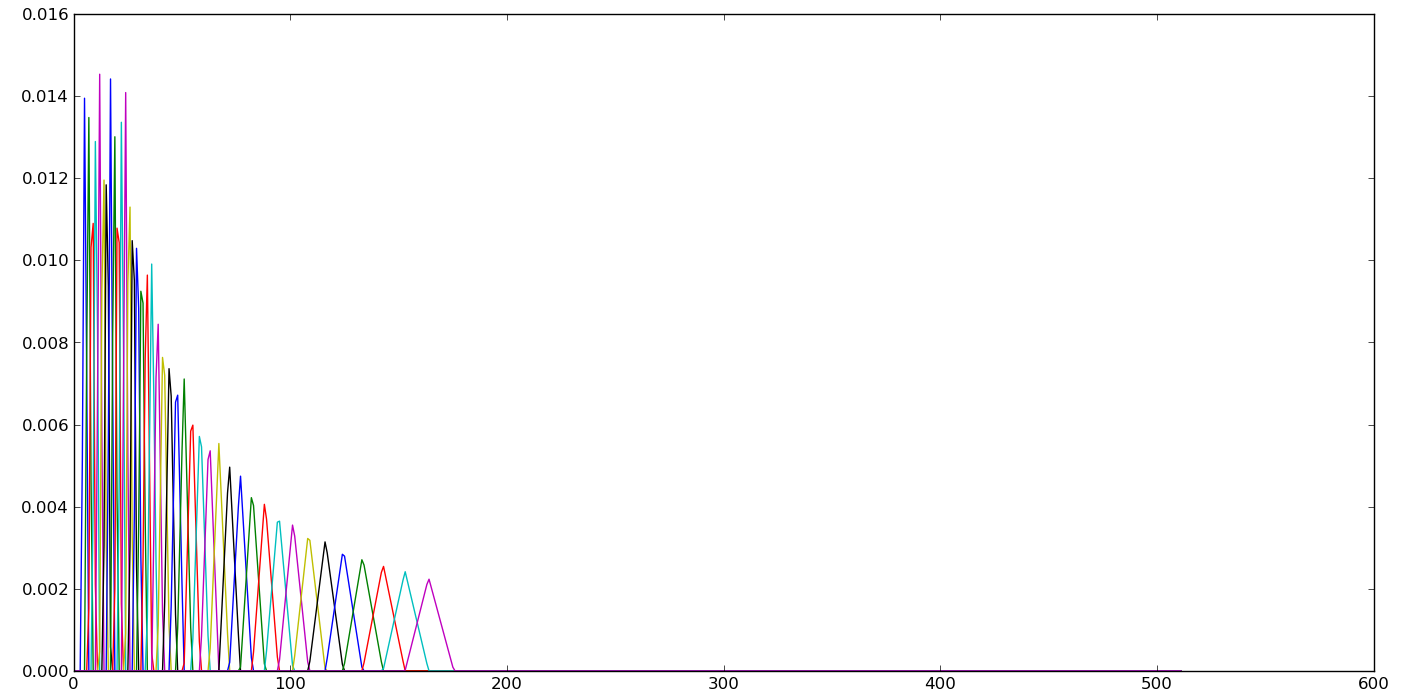
\includegraphics[scale=0.4]{../filterbank.png}
\caption{Mel Filterbank.}
\label{fig:filterbank}
\end{figure}

\begin{figure}
\centering
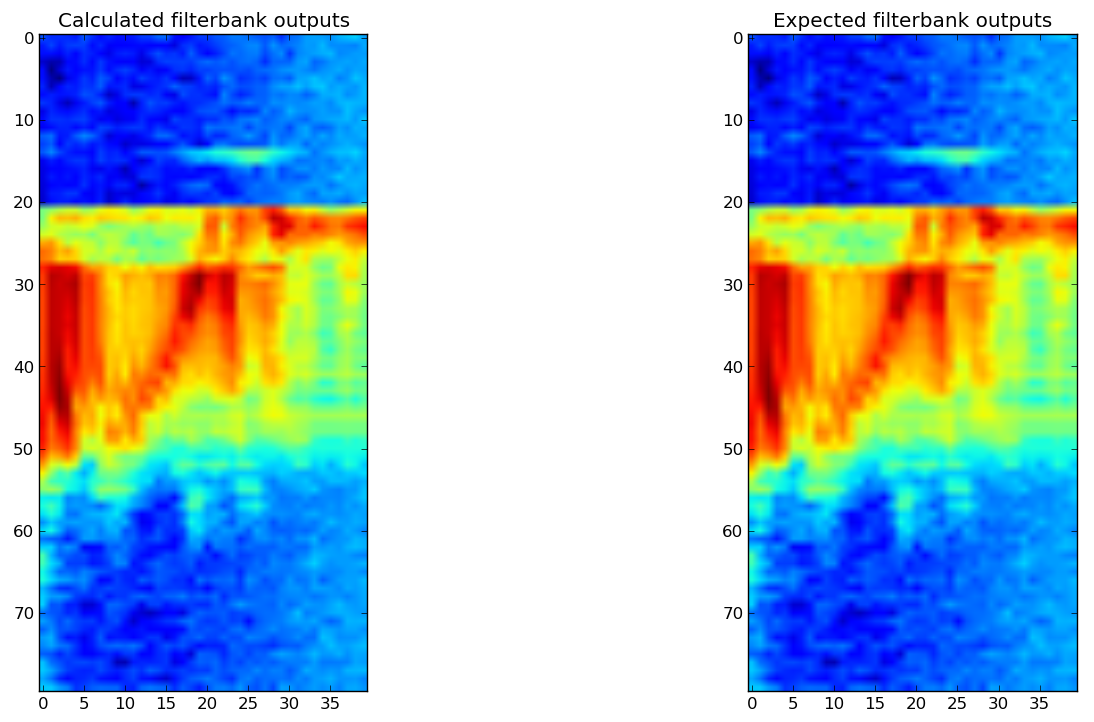
\includegraphics[scale=0.4]{../mspec.png}
\caption{Mel Spectrum.}
\label{fig:mspec}
\end{figure}

\subsection{Cosine Transform}
After applying the Discrete Cosine Transform to the Mel spectrum for thirteen coefficients, we are able to get the MFCCs of the original signal (Fig. \ref{fig:mfcc}).

\begin{figure}
\centering
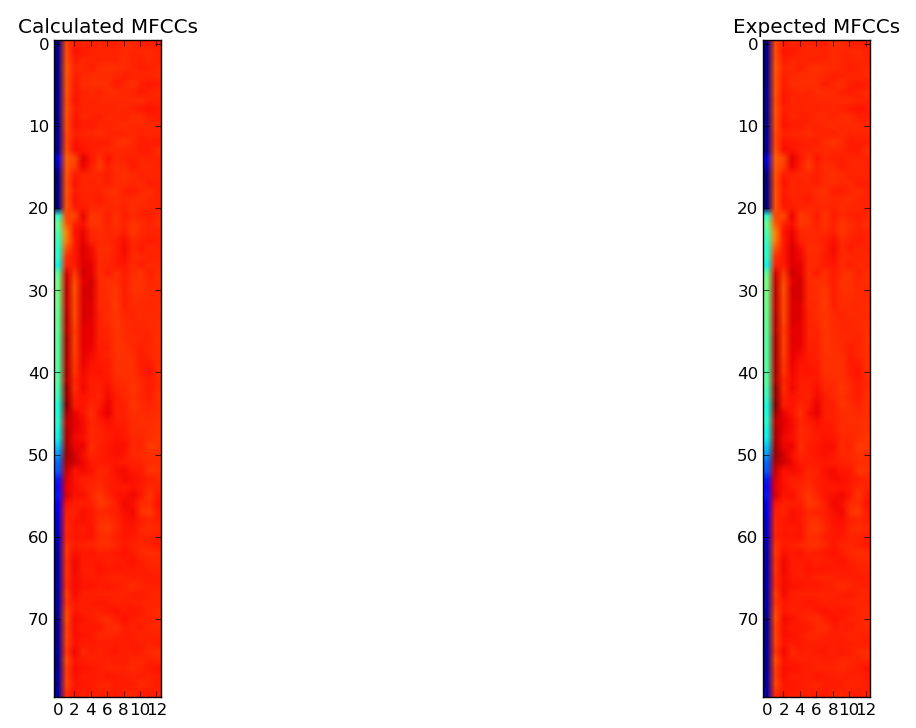
\includegraphics[scale=0.4]{../mfcc.png}
\caption{MFCCs of the Signal.}
\label{fig:mfcc}
\end{figure}

After computing the MFCCs for all the utterances in the $tidigits$, we can see that the differences between various digits and speakers are becoming more apparent. In Figure \ref{fig:mfccs} we see the MFCCs of a man saying ``o'' and ``zero'', whereas on Figure \ref{fig:mfccs1} we see the MFCCs of a man and a woman saying ``o''. By observing these three utterances, we can see that there are some similarities and differences between all three. For example the MFCCs of the utterances of the man, maintain a similar hue, which is probably a result of the tone of the speaker's voice, whereas the utterances of the man and woman speaking the same word, even though they have different hues, they maintain a similar structure, which is a result of the word being uttered.

Of course these characteristics are not so apparent, so as to be able to be classified by a human. But what we can derive of them is the fact that they indeed indicate the speaker or the word being uttered.

\begin{figure}
\centering
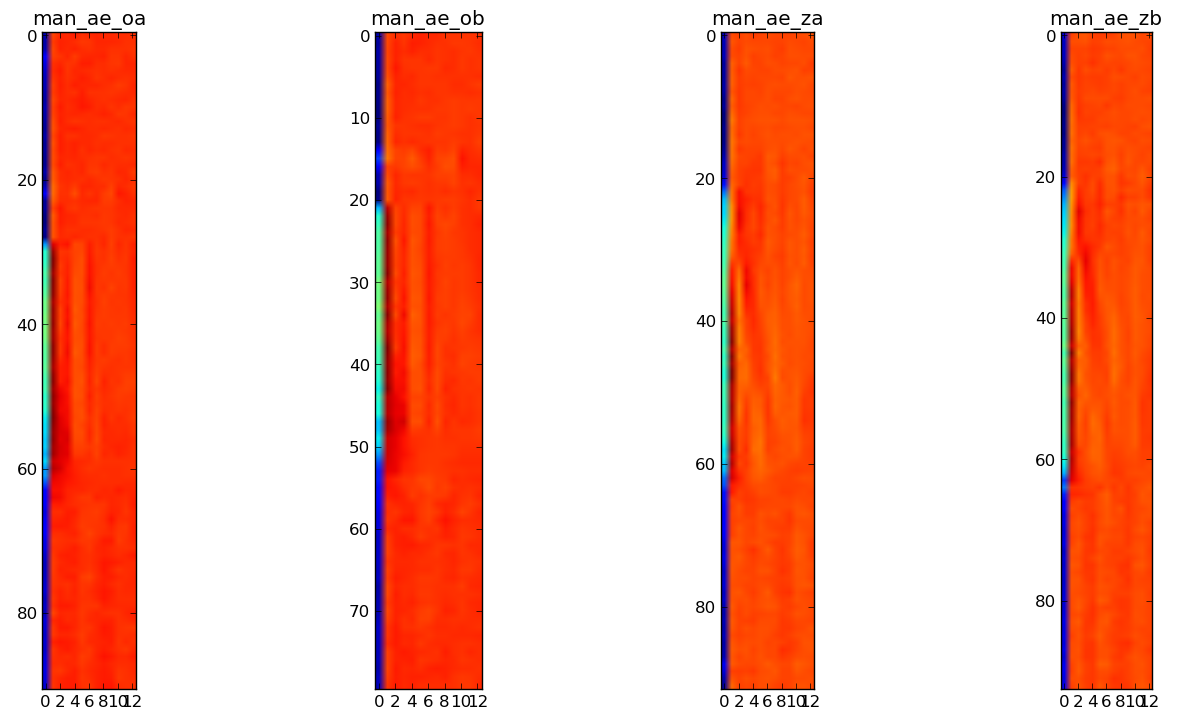
\includegraphics[scale=0.4]{../mfccs.png}
\caption{MFCCs for different utterances.}
\label{fig:mfccs}
\end{figure}

\begin{figure}
\centering
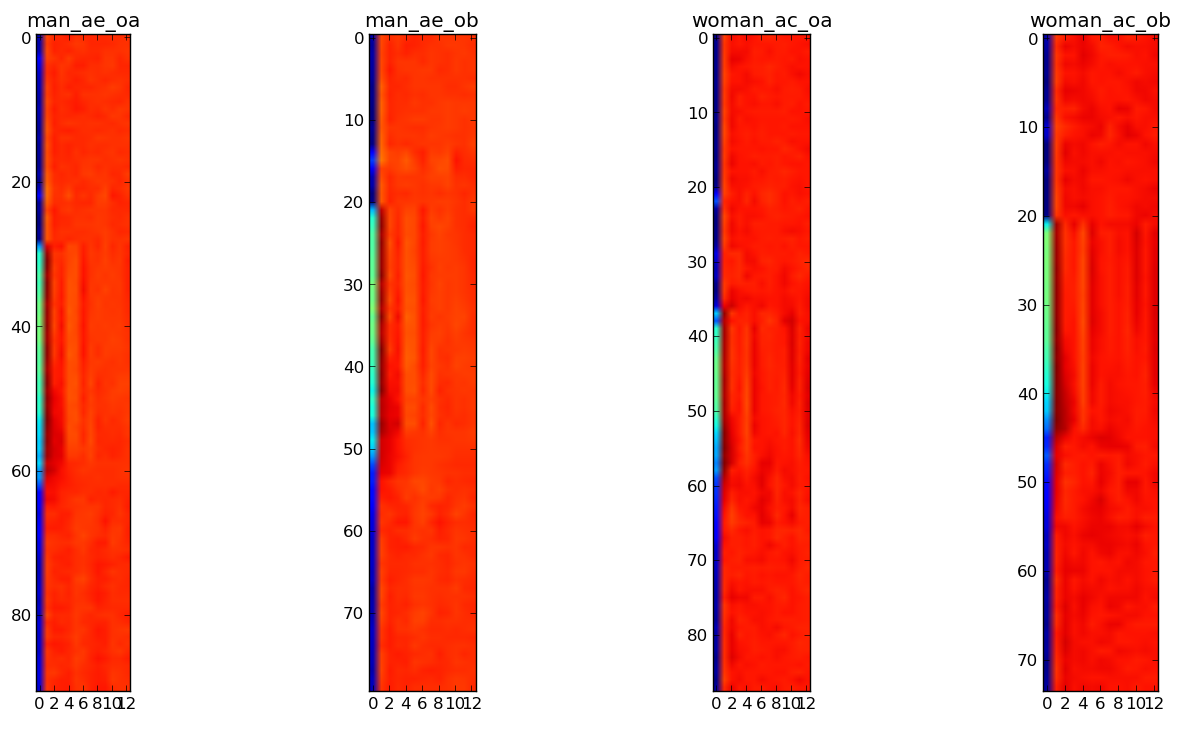
\includegraphics[scale=0.4]{../mfccs1.png}
\caption{MFCCs for different utterances.}
\label{fig:mfccs1}
\end{figure}

\section{Feature Correlation}
The final form of the MFCCs produces a 13-element feature for every frame. By creating the correlation matrix, we can check whether these different features are correlated, i.e. whether they carry similar information or not. Figure \ref{fig:corr} shows the correlations between the 13 elements of the MFCC features. Every element $\rho_{ij}$ of this matrix is the correlation coefficient of the $ith$ and $jth$ element of the feature. It is calculated by the following expression:

\begin{equation}
\rho_{ij} = \dfrac{Cov(i, j)}{\sigma_i \sigma_j}
\end{equation}
where $Cov(i, j)$ is the covariance of $i$ and $j$ and $\sigma$ is the variance. The correlation coefficient is bound within $[-1 \dots 1]$. When $\rho_{ij} > 0$, then $i$ and $j$ are said to be positively correlated, when $\rho_{ij} < 0$ they are negatively correlated and when $\rho_{ij} = 0$ then they are uncorrelated.

If two elements are found to be highly correlated (positively or negatively), it means that they behave in a very similar or foreseeable manner within a large number of observations. Hence the existence of both is redundant, since we don't gain new information by using both of them and one could be dropped.

The matrix in Figure \ref{fig:corr} has a diagonal of ones, which is to be expected, since the diagonal gives the correlation between every element with itself. We can see that there is a quite high correlation between element 1 and 2, which could mean that they carry similar information. Other than that, all other elements are very lowly correlated or completely uncorrelated. By comparing this matrix to the matrix of Figure \ref{fig:corr1}, which shows the correlations between the filterbank features, we can see that the computation of the Discrete Cosine Transform results in a significant improvement of the feature. It not only reduces the dimension of the feature to almost one fourth, but it is obvious that the elements of the filterbank features are very highly correlated (with very few exceptions of uncorrelated elements).

In the end we are left with a compact and ``information-rich'' feature. This completely justifies the use of diagonal covariance matrices for Gaussian modelling, since the covariance matrix is a metric very similar to the correlation matrix.


\begin{figure}
\centering
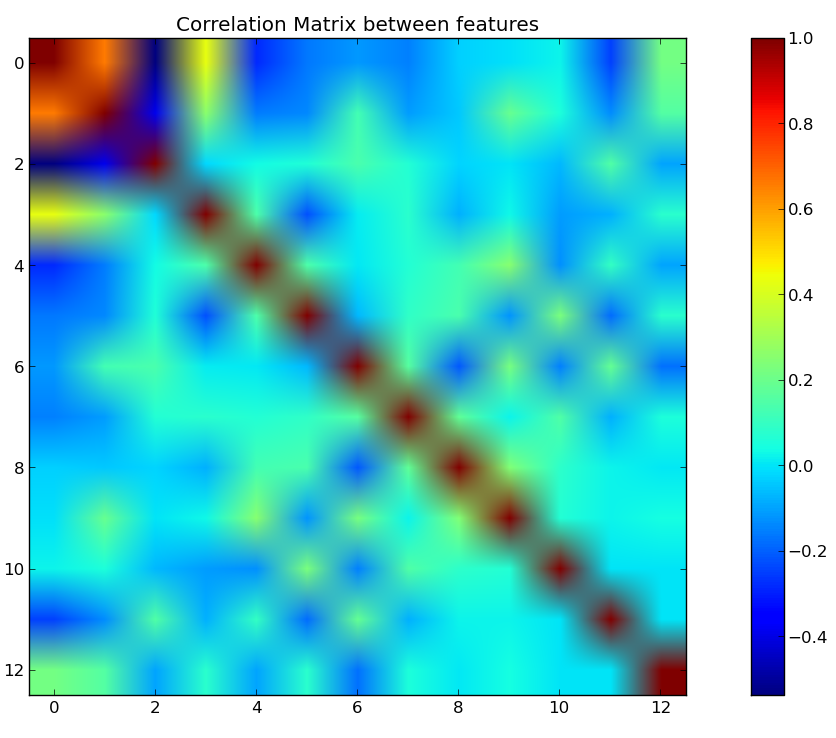
\includegraphics[scale=0.4]{../correlation.png}
\caption{Correlation Matrix of features.}
\label{fig:corr}
\end{figure}

\begin{figure}
\centering
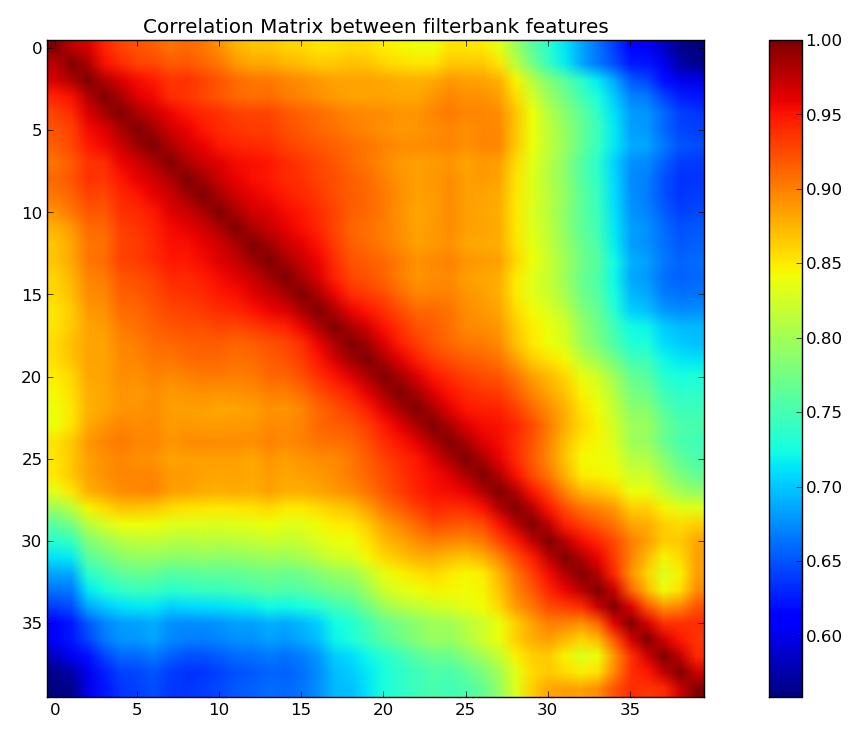
\includegraphics[scale=0.4]{../correlation1.png}
\caption{Correlation Matrix of filterbank features.}
\label{fig:corr1}
\end{figure}

\section{Gaussian Mixture Models}
After training a Gaussian Mixture Model (GMM) on the features that were produced in the previous tasks, we are able to calculate the probability of each frame ``belonging'' to each of the Gaussians. By observing these probabilities we can monitor the different patterns that emerge.

In Figures \ref{fig:probs} and \ref{fig:probs1} we can see similarities between speakers and words. In these patterns (a man saying ``o'' and ``zero'' and a woman saying ``o'') some similarities between the speaker and the word are again visible. Of course these are only human observations of very few examples, but if we compare these to Figures \ref{fig:mfccs} and \ref{fig:mfccs1} we can see that now there are more obvious similarities between the images with the same speaker saying the same word. In a way the different speakers are starting to separate, even when speaking the same words.


\begin{figure}
\centering
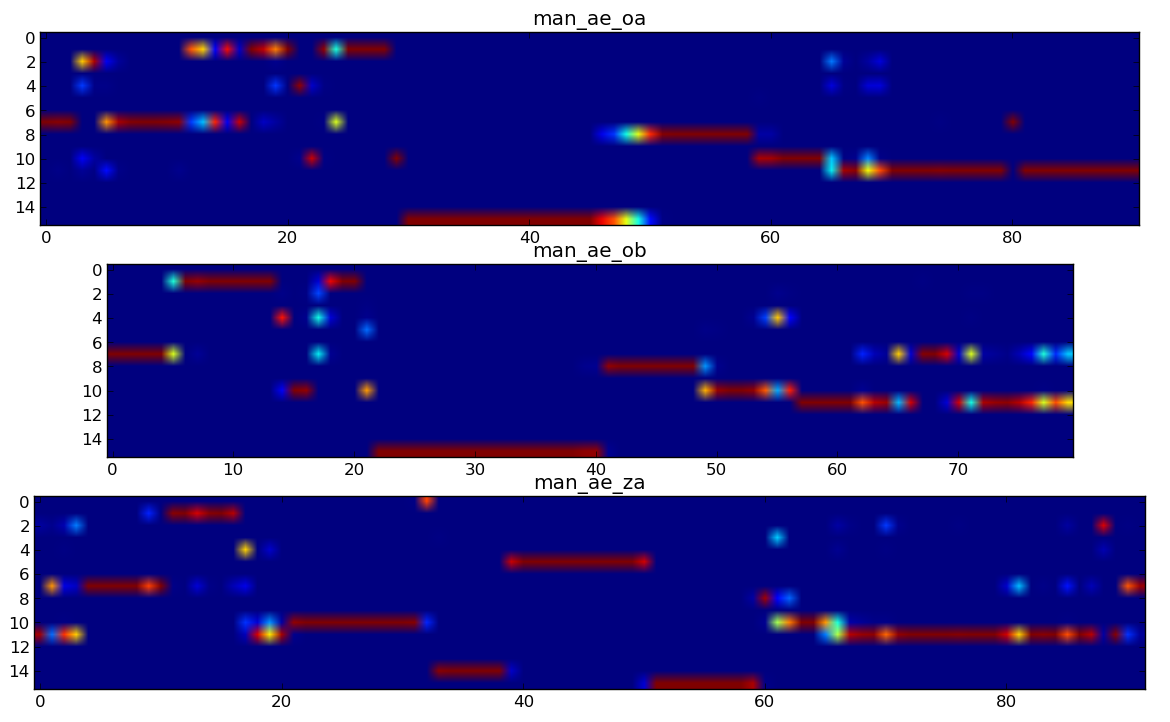
\includegraphics[scale=0.5]{../probs.png}
\caption{Posterior probabilities per frame and Gaussian model for different utterances.}
\label{fig:probs}
\end{figure}

\begin{figure}
\centering
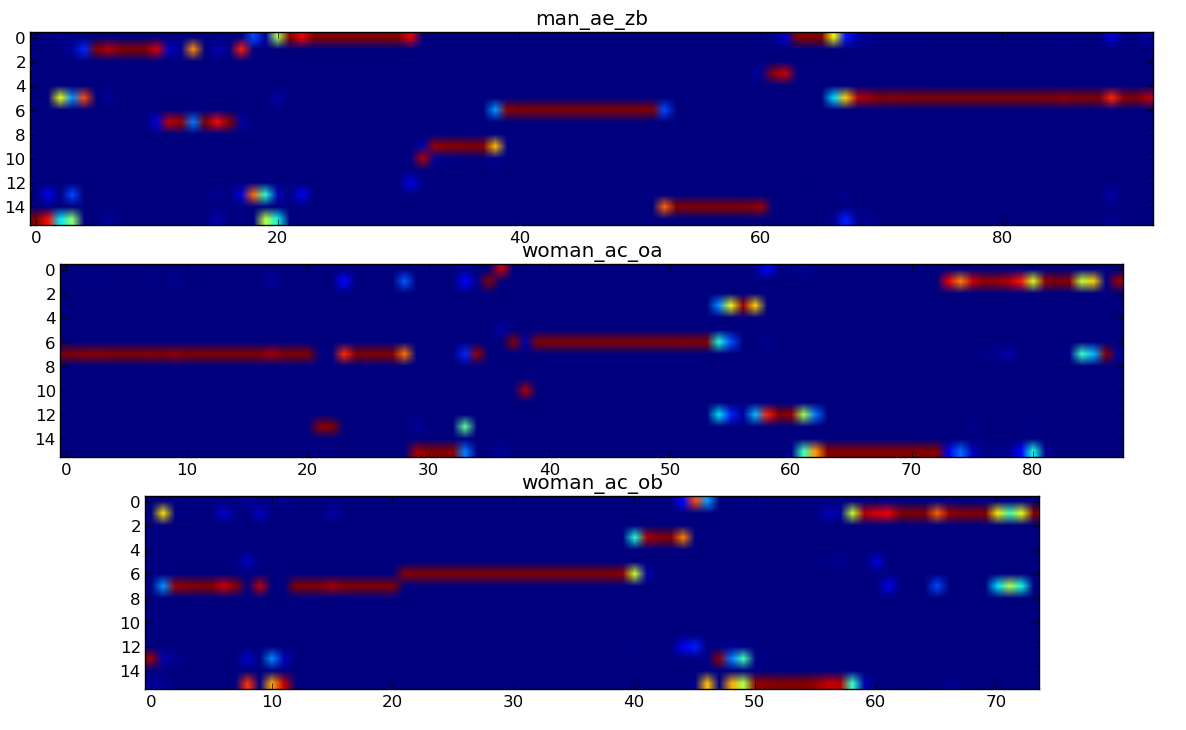
\includegraphics[scale=0.5]{../probs1.png}
\caption{Posterior probabilities per frame and Gaussian model for different utterances.}
\label{fig:probs1}
\end{figure}

\section{Comparing Utterances}
After calculating the local Euclidean distances between the MFCC features and global distances of different utterances the distance matrix was created and printed. The result is shown in Figure \ref{fig:glob}. The diagonal of the matrix plus the neighbouring elements (that is, a $2 \times 2$ square matrix, whose diagonal is the large matrix's diagonal) seem to have the shortest distances (dark blue). Since every two utterances are the same speaker saying the same digits, the results of the distance matrix are very good. It is obvious that there is a separation of utterances based on the speaker as well as the digit.

There are of course other areas in the matrix with short distances (light blue areas), that indicate that these utterances are found to be similar. These utterances are usually the same digit uttered by a different speaker (e.g. utterances 8, 9, 30 and 31 which are the digit 3 uttered by the man and the woman). This means that sometimes, there is a better distinction between the digit and not so much of the speaker.

However, looking at the dendrogram in Figure \ref{fig:dendro} the interesting thing to observe is, the fact that, the leaf nodes that are paired are always utterances of the same speaker \textbf{and} digit. The only exception is the woman saying ``zero'', where the two leaf nodes end up being connected at a higher level, which could probably indicate that the algorithm found similarities to other utterances to be more significant. At the second level of the tree in many cases the nodes that are connected, lead to the same digit (e.g. the node leading to a man saying ``five'' is connected to the node leading to a woman saying ``five''). In other cases we can see that different utterances of the same speaker are grouped together. This indicates that both characteristics of the utterance are significant and influence the classification. However this is a very small dataset, so it is not easy to draw conclusions.

When using standardized data (remove the global mean and divide by the global standard deviation of the MFCCs) we get the results of Figure \ref{fig:glob_std}. It is obvious in this Figure that the use of standardized data does not affect the relative distances between the utterances (the colors of the image remained intact). However we can see that the numbers have decreased. This means that the global distances between the utterances have all been scaled down, but their relative ``positions'' have not changed. The dendrogram produced by this dataset is exactly the same as the one in Figure \ref{fig:dendro}.

Finally the GMM probabilities were used and produced the results seen in Figures \ref{fig:glob_probs} and \ref{fig:dendro_probs}. We can see that with this dataset, the image has changed significantly. Even though the diagonal remains the same, there are now many more large distances between utterances (colours yellow, orange and red). However we can also observe that there are also many more small distances (light and dark blue areas). It looks like all the areas that were on the borderline of ``large'' or ``small'' distance (light green areas), are now pushed up or down. The dendrogram has a new form as well. The first thing that changes is that now, not all utterances are paired up correctly at the leaf nodes. It is also very interesting that in this dendrogram, when starting from the root node, the utterances are divided into two groups based on the speaker (there are only two speakers in this dataset), which did not happen before.

As a general estimation I believe that using the probabilities instead of the MFCCs deteriorates the system. However a conclusion cannot be reached without a proper dataset and the without the use of the appropriate metrics.

\begin{figure}
\centering
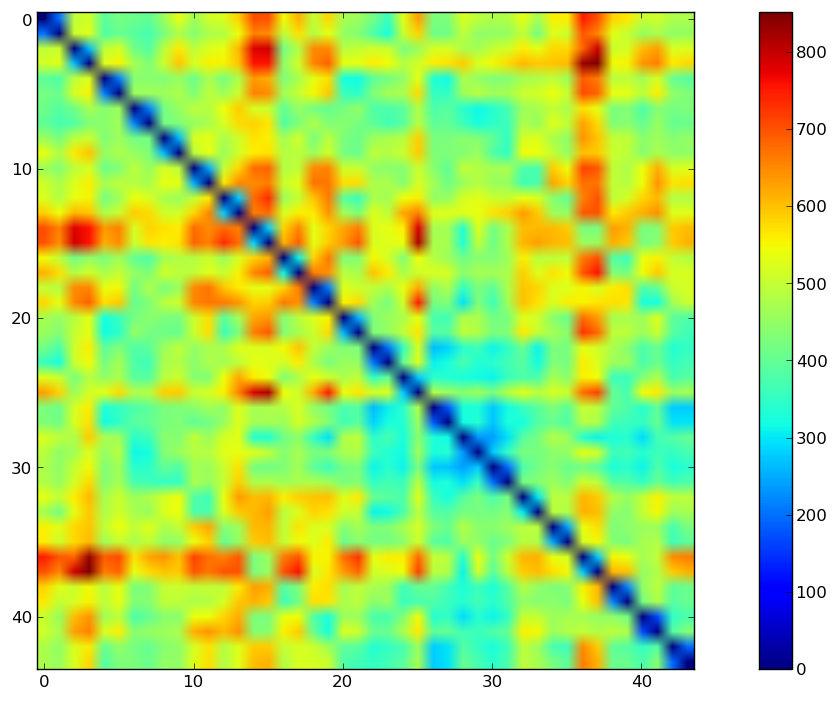
\includegraphics[scale=0.5]{../global_distances_colorbar.png}
\caption{Global distances between different utterances.}
\label{fig:glob}
\end{figure}

\begin{table}
\caption{Order of the utterances}
\label{tab:utt}
\centering
\footnotesize
    \begin{tabular}{cc}
    0 man\_ae\_oa & 22 woman\_ac\_oa\\
    1 man\_ae\_ob & 23 woman\_ac\_ob\\
    2 man\_ae\_za & 24 woman\_ac\_za\\
    3 man\_ae\_zb & 25 woman\_ac\_zb\\
    4 man\_ae\_1a & 26 woman\_ac\_1a\\
    5 man\_ae\_1b & 27 woman\_ac\_1b\\
    6 man\_ae\_2a & 28 woman\_ac\_2a\\
    7 man\_ae\_2b & 29 woman\_ac\_2b\\
    8 man\_ae\_3a & 30 woman\_ac\_3a\\
    9 man\_ae\_3b & 31 woman\_ac\_3b\\
    10 man\_ae\_4a & 32 woman\_ac\_4a\\
    11 man\_ae\_4b & 33 woman\_ac\_4b\\
    12 man\_ae\_5a & 34 woman\_ac\_5a\\
    13 man\_ae\_5b & 35 woman\_ac\_5b\\
    14 man\_ae\_6a & 36 woman\_ac\_6a\\
    15 man\_ae\_6b & 37 woman\_ac\_6b\\
    16 man\_ae\_7a & 38 woman\_ac\_7a\\
    17 man\_ae\_7b & 39 woman\_ac\_7b\\
    18 man\_ae\_8a & 40 woman\_ac\_8a\\
    19 man\_ae\_8b & 41 woman\_ac\_8b\\
    20 man\_ae\_9a & 42 woman\_ac\_9a\\
    21 man\_ae\_9b & 43 woman\_ac\_9b \\
    \end{tabular}
\end{table}


\begin{figure}
\centering
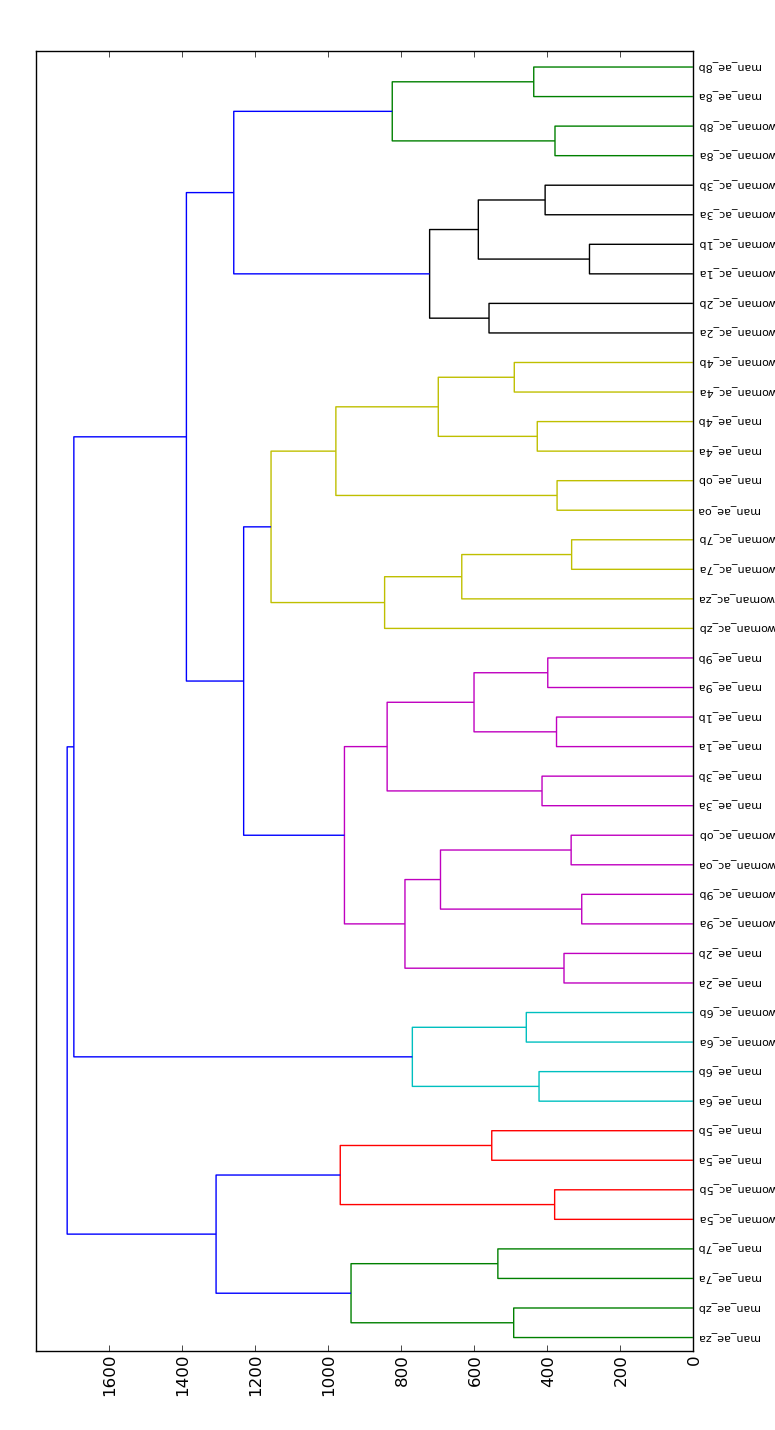
\includegraphics[scale=0.4]{../dendrogram.png}
\caption{Results of the hierarchical clustering based on the global distances.}
\label{fig:dendro}
\end{figure}

\begin{figure}
\centering
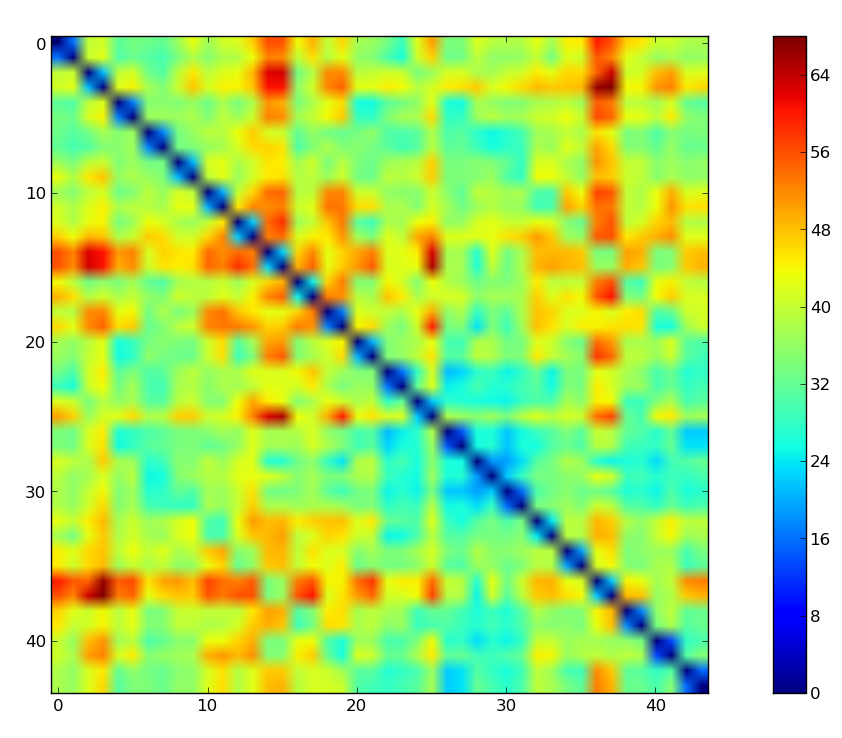
\includegraphics[scale=0.45]{../D_std.png}
\caption{Global distances between different utterances using standardized data.}
\label{fig:glob_std}
\end{figure}

\begin{figure}
\centering
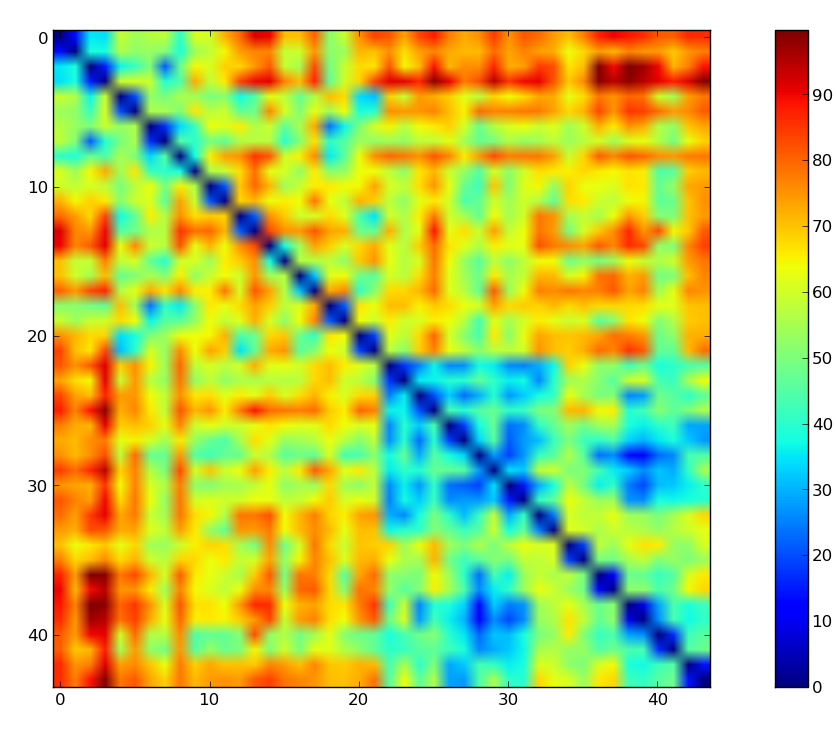
\includegraphics[scale=0.45]{../D_probs.png}
\caption{Global distances between different utterances using the GMM posteriors.}
\label{fig:glob_probs}
\end{figure}

\begin{figure}
\centering
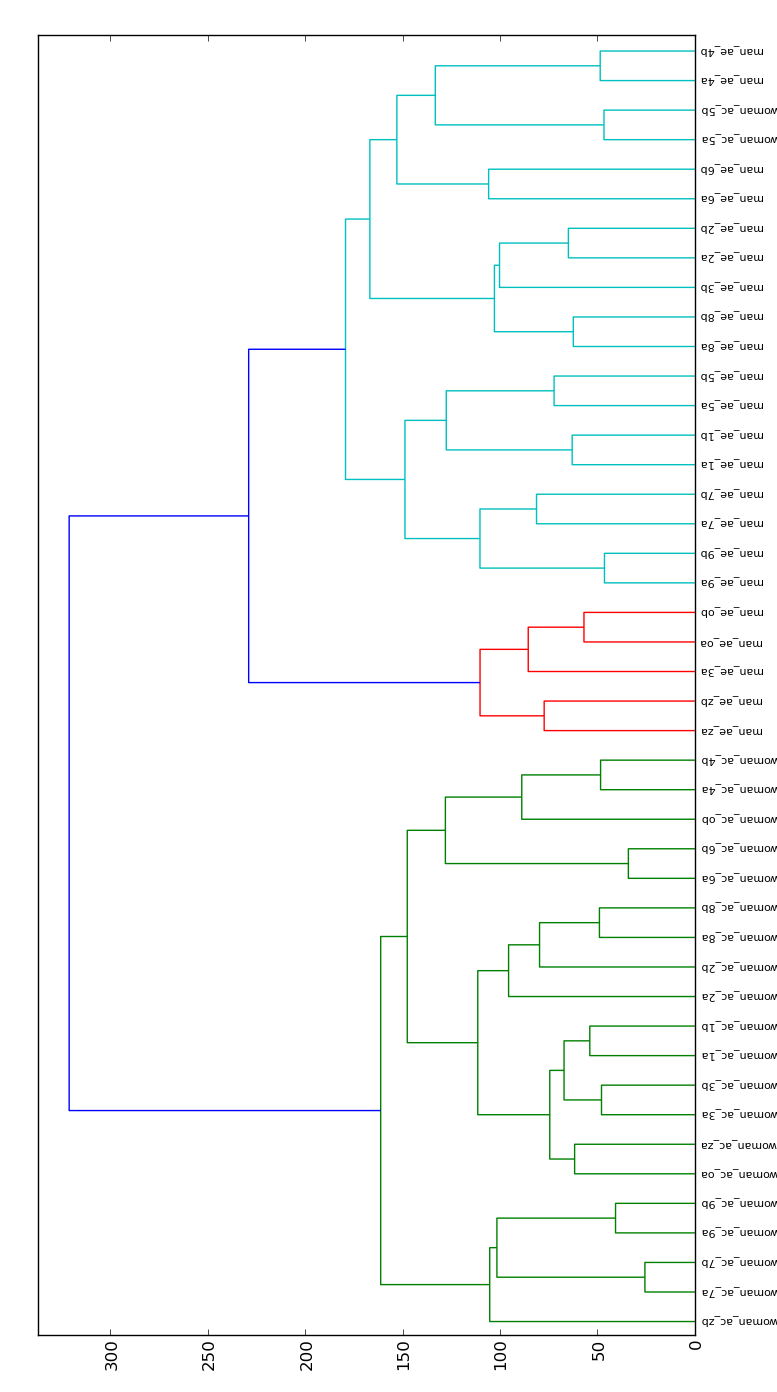
\includegraphics[scale=0.4]{../dendrogram_probs.png}
\caption{Results of the hierarchical clustering based on the global distances of the GMM posteriors.}
\label{fig:dendro_probs}
\end{figure}

\end{document}